\section*{Реализация}
\addcontentsline{toc}{section}{Реализация}

\subsection*{Модель сущность-связь}
\addcontentsline{toc}{subsection}{Модель сущность-связь}

Первым делом необходимо формализовать таблицы базы данных. Опишем нужные таблицы:

\begin{itemize}
	\item Textbook -- таблица с книгами в формате BibTeX. Обладает несколькими UNIQUE столбцами:
	      \begin{itemize}
	      	\item ident -- идентификатор книги, должен быть уникальным, так как именно
	      	      он используется для идентификации библиографической ссылки в стандарте LaTeX.
	      	\item isbn -- уникальный для каждой книги ключ, позволяет исключить дублирование.
	      \end{itemize}
	\item LiteratureList -- таблица, хранящая списки литературы. Имеет UNIQUE ограничение на
	      пару из ID курса, которому присвоен список и года этого курса. Это необходимо для
	      идентификации списка литературы.
	\item Literature -- так называемая таблица пересечения, необходимая для создания связи
	      многие-ко-многим между таблицами LiteratureList и Textbook.
	\item Course -- задает учебный курс. Стоит отметить, что один учебный курс может иметь
	      несколько списков литературы за разные года. Имеет ссылки на кафедру, к которой 
	      привязан и лектора, читающего курс. Обладает UNIQUE ограничением на тройку из
	      названия, кафедры и семестра, в котором читается курс.
	\item Department -- задает кафедру, имеет UNIQUE поле title, характеризующее
	      название кафедры.
	\item Lecturer -- хранит всех лекторов. Однозначно идентифицируется именем и датой рождения.
\end{itemize}

Все таблицы обладают суррогатными первичными ключами.

Стоит также отметить два важных решения, которые были приняты для всей базы данных.

Во-первых, каждая запись имеет поле timestamp -- временную метку добавления или изменения записи.
Это позволит иметь историю изменений. Также нужно уточнить, что данное поле имеет тип integer,
что является более общим решением, чем хранение метки во внутреннем формате СУБД.

Во-вторых, в базе данных будет отсутствовать возможность удаления записи. Для этого каждая
запись имеет флаг isDeleted. При удалении пользователем записи она будет помечаться, как удаленная.
У данного решения есть ряд преимуществ. Это позволяет обезопасить базу данных от ошибок пользователя
и от потенциального взлома системы. И в том, и в другом случае никому не удастся нанести
непоправимый ущерб данным. Причем блокировка будет осуществляться за счет того, что у учетной записи,
через которую пользователь будет взаимодействовать с базой данных, не будет прав на удаление из базы данных.
При этом все равно будет администратор, у которого данная возможность есть.

В итоге получаются диаграмма модели сущность-связь, показанная на рисунке ~\ref{ris:ermodel}.

\begin{figure}[h!]
	\center{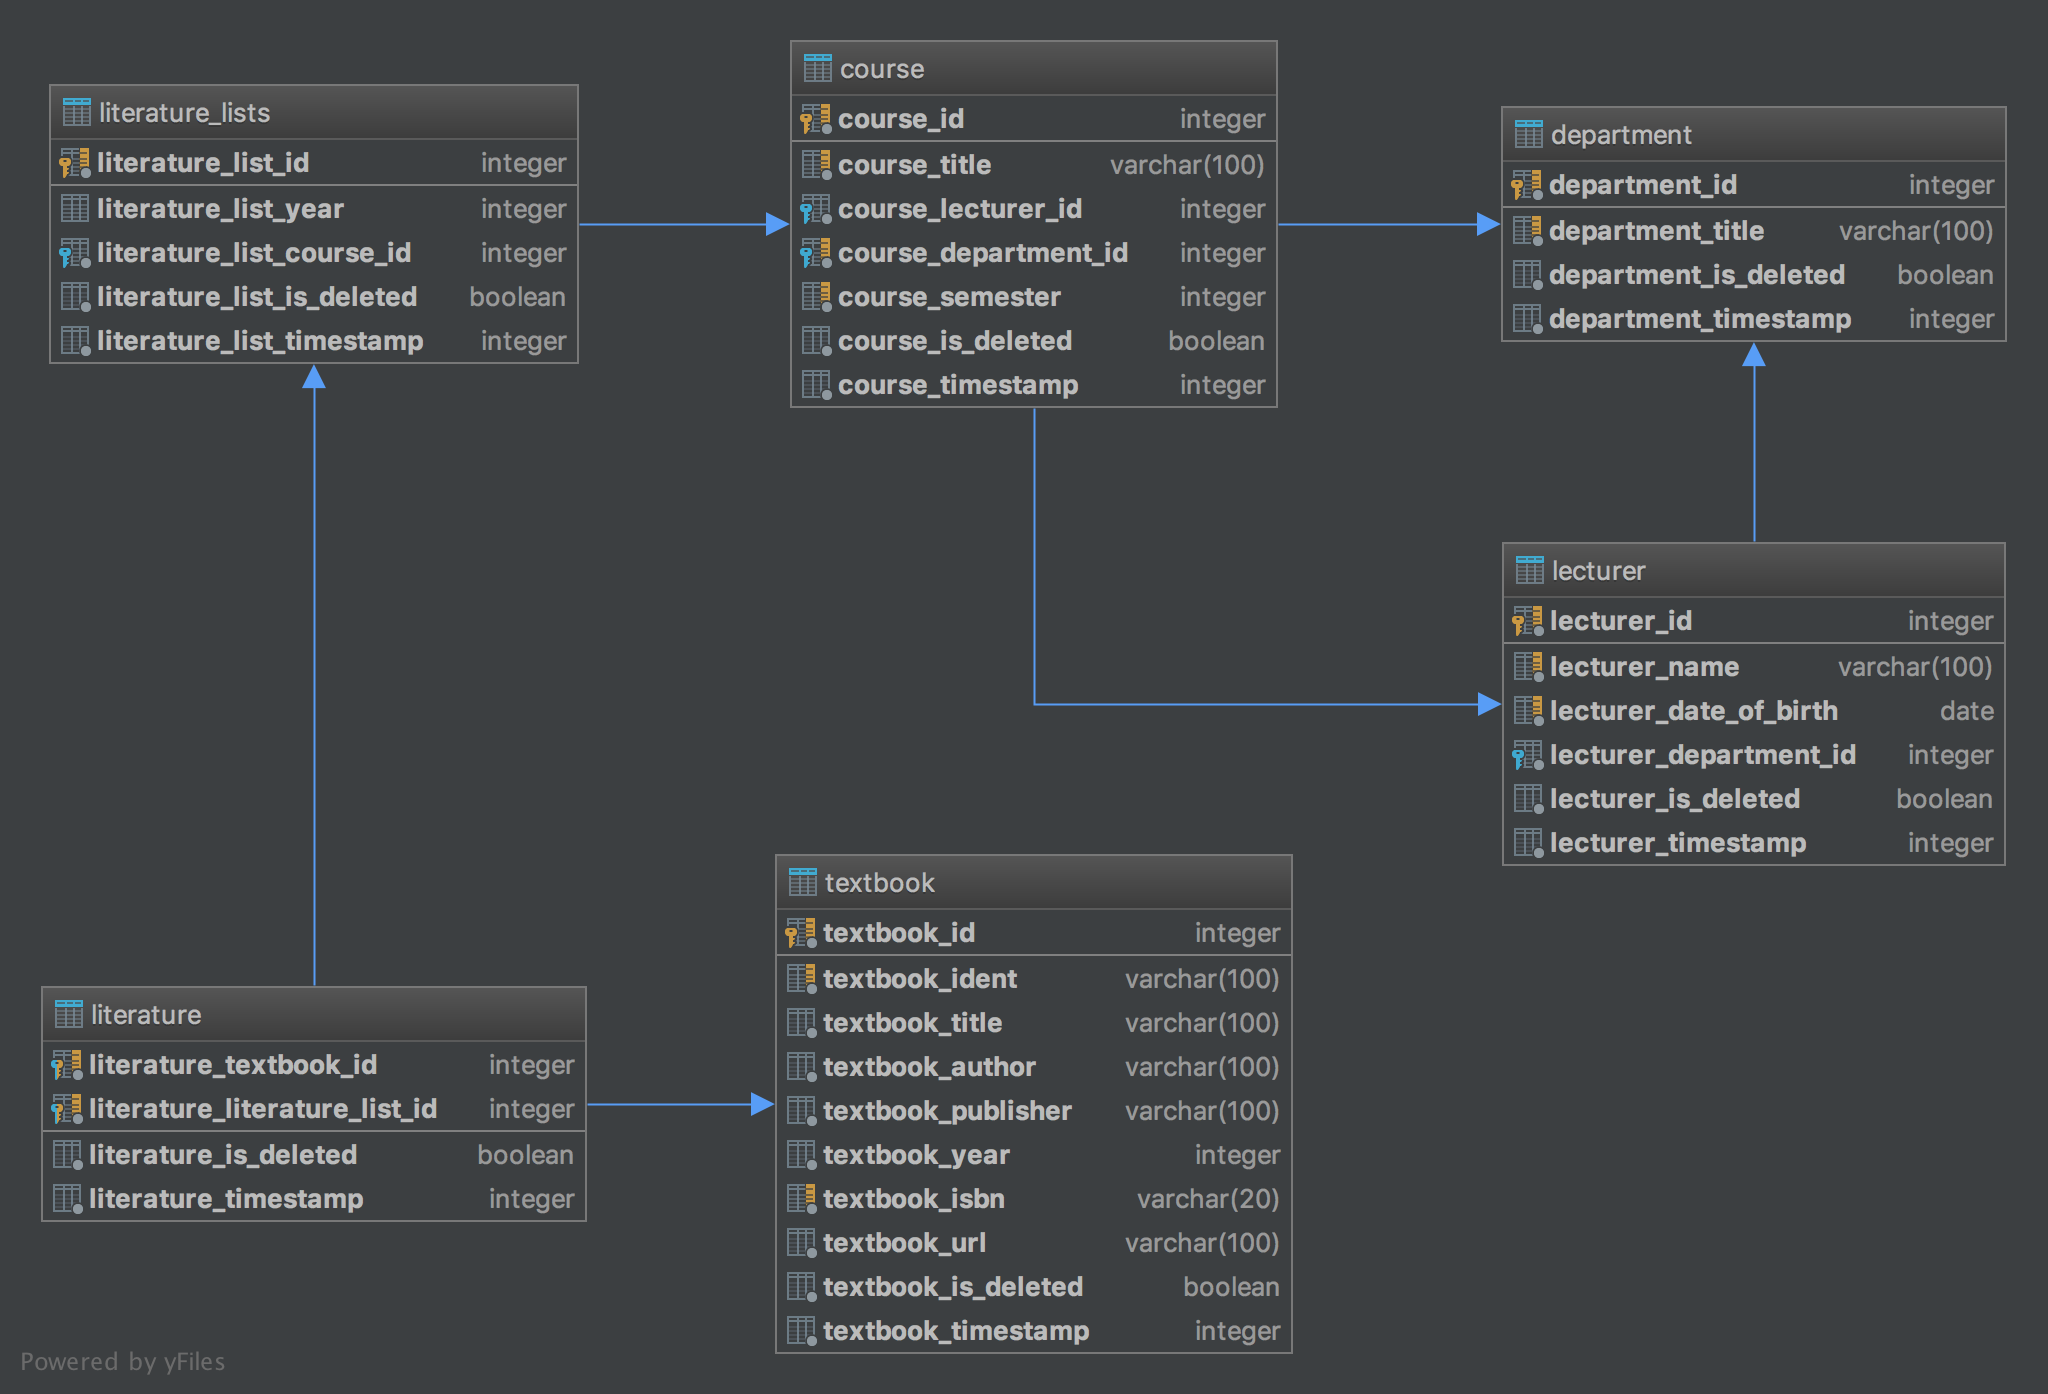
\includegraphics[width=1\linewidth]{schema.png}}
	\caption{Диаграмма модели сущность-связь}
	\label{ris:ermodel}
\end{figure}

Стоит отдельно отметить минимальные кардинальные связи в этой базе данных. Для упрощения конфигурации серверной части предполагается 
запрет любым пользователям, кроме администратора, какого-либо удаления. Удаление предполагается каскадное, реализованное на серверной части
с помощью обновления флага isDeleted. Таким образом, везде неявно предполагается минимальная кардинальная связь единица.

В качестве альтернативного решения можно было бы использовать триггеры, которые вместо удаления будут
производить обновление поля. Но в таком случае пострадает переносимость. Дело в том, что не в каждой
SQL базе данных присутствуют гибкие настройки прав и будет уже не так легко заменить базу данных.
На уровне серверной части работа с базой данной реализована через стандартную библиотеку для работы с
SQL, что дает возможность будущей миграции на любую SQL базу данных. Более подробно реализация будет описана ниже.
В то время как предложенный подход не имеет такой завязки на настройку прав пользователей.

Выбор максимальных кардинальных связей основан исключительно на функциях таблиц, описанных выше и предполагаемой
логики. Объясним выбор этих связей:

\begin{itemize}
	\item Department-Lecturer -- предполагается, что преподаватель может числиться только на одной кафедре, а у кафедры 
	      может быть много преподавателей,
	\item Department-Course -- аналогично случаю Department-Lecturer,
	\item Lecturer-Course -- обычно в университетских программах при наличии нескольких преподавателей в учебном
	      курсе главным считается лектор, так как именно он определяет программу курса, а значит и его список литературы. 
	      Таким образом, для идентификации курса достаточно одного преподавателя -- лектора. С другой стороны, лектор может
	      вести несколько учебных курсов.
	\item Course-LiteratureList -- у каждого курса может быть несколько разных списков литературы за разные года, но
	      у каждого списка только один курс,
	\item LiteratureList-Literature-Textbook -- связь многие-ко-многим между LiteratureList и Textbook, так как
	      каждый список содержит множество книг, а учебник может быть использован в нескольких курсах.
\end{itemize}

\subsection*{Интерфейс программирования приложений}
\addcontentsline{toc}{subsection}{Интерфейс программирования приложений}

При рассмотрении интерфейсов программирования приложений была описана архитертура REST. Согласно
этой архитектуре каждый метод должен принимать всю необходимую информацию
для выполнения запроса. Таким образом, для каждого вида данных был реализован следующий набор методов:

\begin{itemize}
    \item add -- POST запрос, содержащий данные для добавления в теле,
    \item get -- GET запрос, получающий данные от приложения,
    \item prototype -- GET запрос, получающий прототип JSON-файла для искомой таблицы.
\end{itemize}

Также были реализованы две дополнительных команды: report и migrate.

Первая получает данные, необходимые для однозначной идентификации требуемого списка литературы
и генерирует для этого списка литературы файл в формате BibTeX. 

Команда migrate выполняет копирование списка литературы с одного года на другой. Это необходимо для того,
чтобы облегчить работу пользователя, ведь обычно учебные программы слабо меняются от года к году.

\subsection*{Интерфейс командной строки}
\addcontentsline{toc}{subsection}{Интерфейс командной строки}

Как уже было сказано выше, для интерфейсов командной строки крайне важна автоматизируемость.
Это делает невозможным использование так называемого интерактивного ввода. Другими словами,
любое действие пользователя должно совершаться за один вызов приложения. В результате
было решено использовать следующий подход к проектированию интерфейса: для каждого вида данных,
с которыми будет работать приложение, будет реализована собственная команда. И для каждой такой
команды будет реализован набор подкоманд, выполняющих необходимые действия. В общем случае
команду приложения командной строки можно описать в следующем виде:

\begin{itemize}
    \item prototype -- данный метод добавляет новый файл в файловую систему,
        который содержит в себе прототип для нужного вида данных. После чего пользователь
        должен заполнить этот прототип информацией, которую хочет добавить,
    \item add -- сохраняет данные в приложение,
    \item get -- позволяет получить данные из приложения, можно конфигурировать
        флагами.
\end{itemize}

Также отличительной чертой хорошего приложения командной строки является грамотно оформленная справка.
Рисунок ~\ref{ris:help_example} показывает результат выполнения команды help. 

\begin{figure}[h!]
    \center{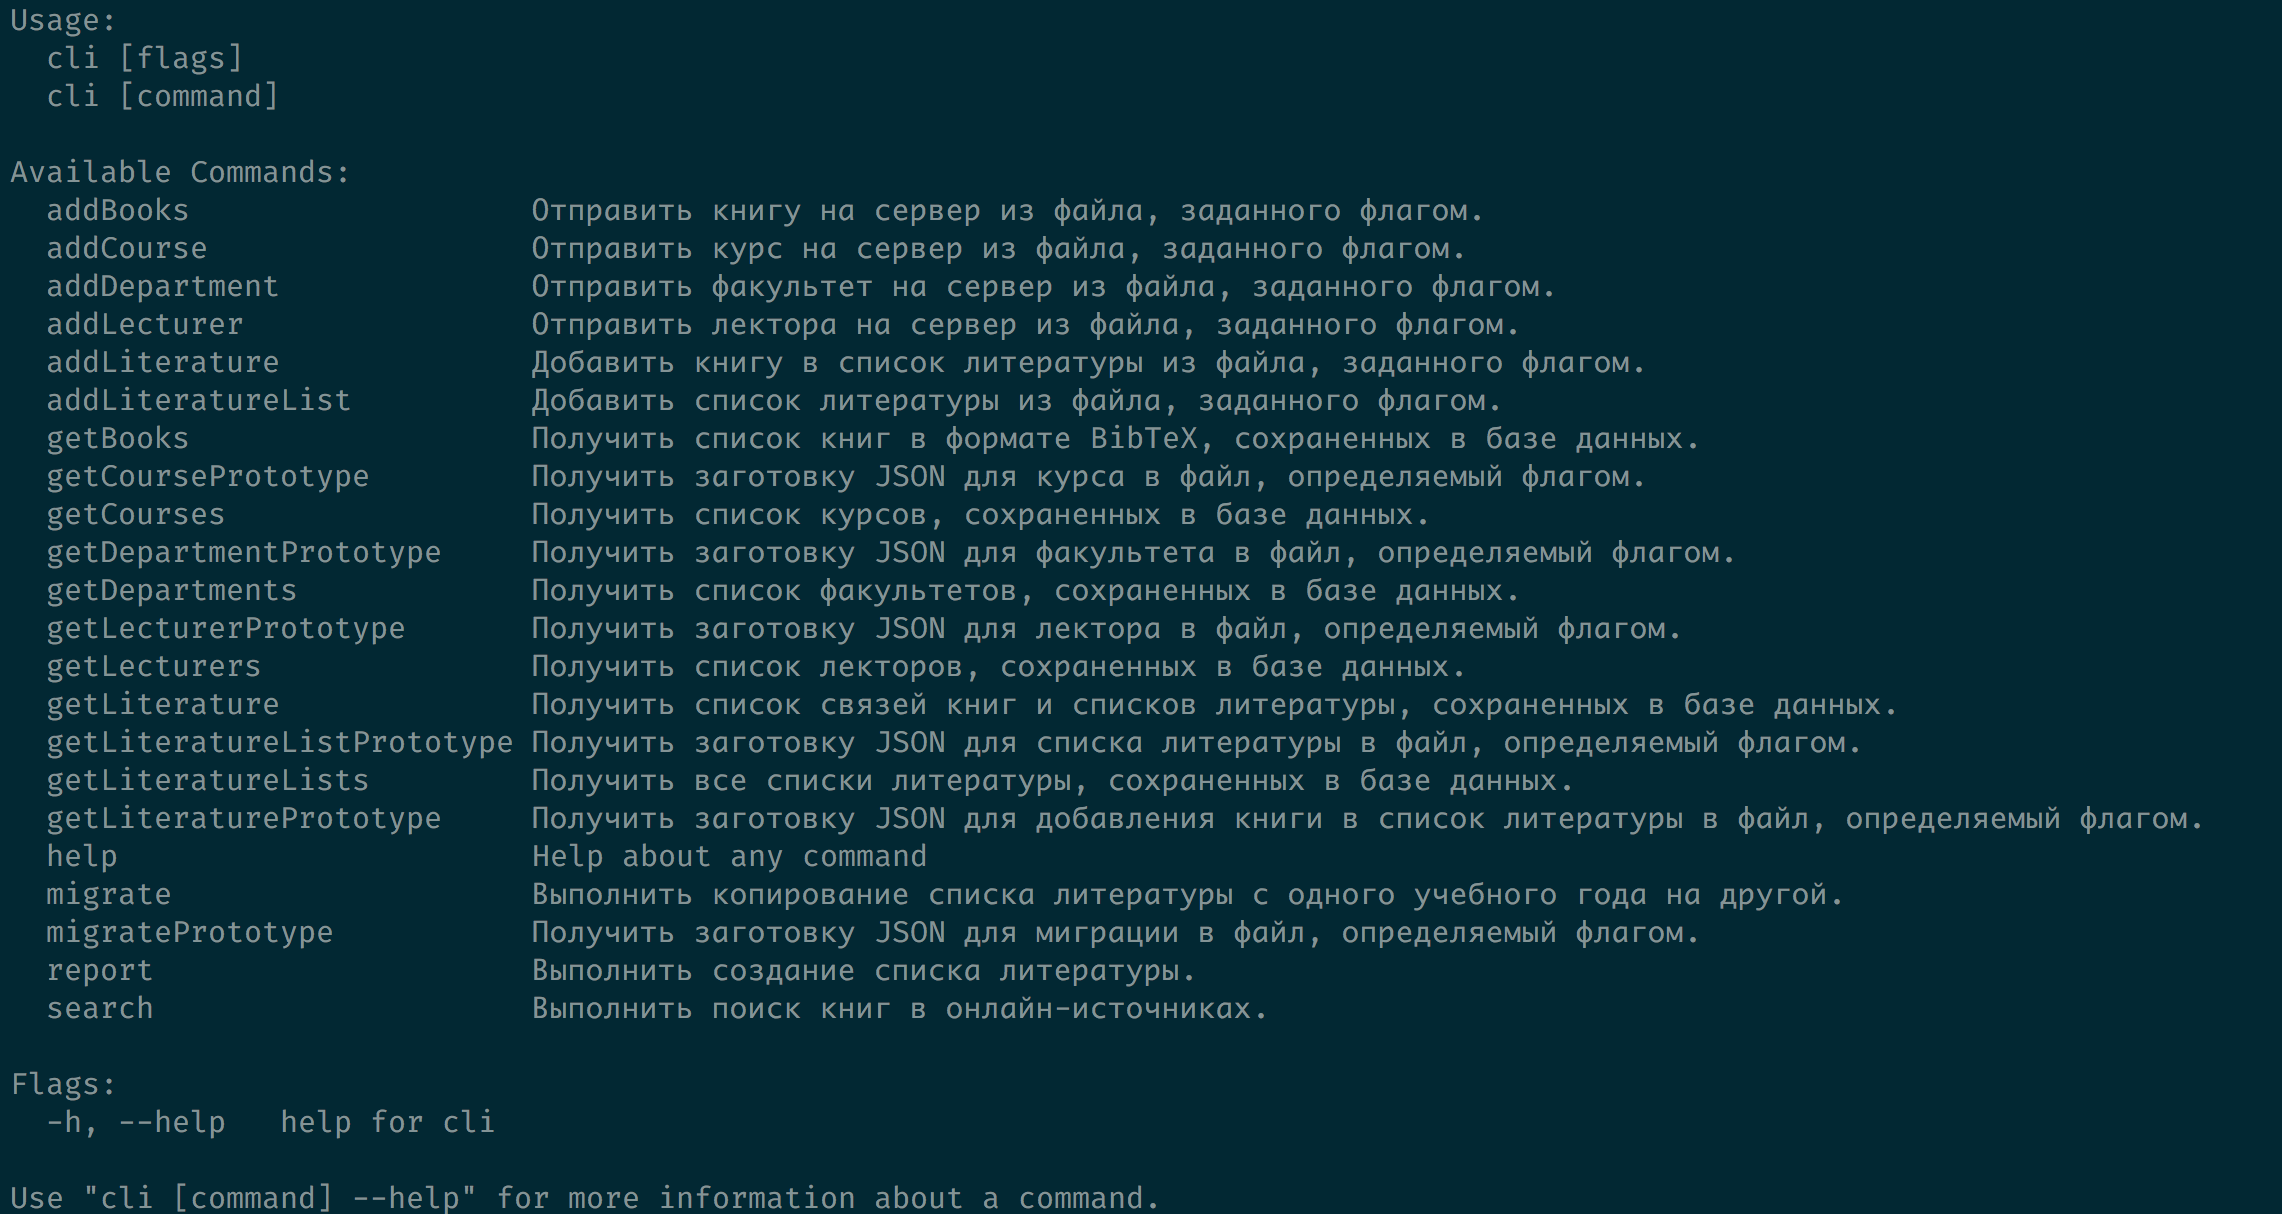
\includegraphics[width=1\linewidth]{help}}
    \caption{Пример работы команды help.}
    \label{ris:help_example}
\end{figure}

Для каждой отдельной команды реализован
отдельный флаг --help, который показывает справку для конкретной команды, что можно видеть на рисунке 
~\ref{ris:help_book_example}. 

\begin{figure}[h!]
\center{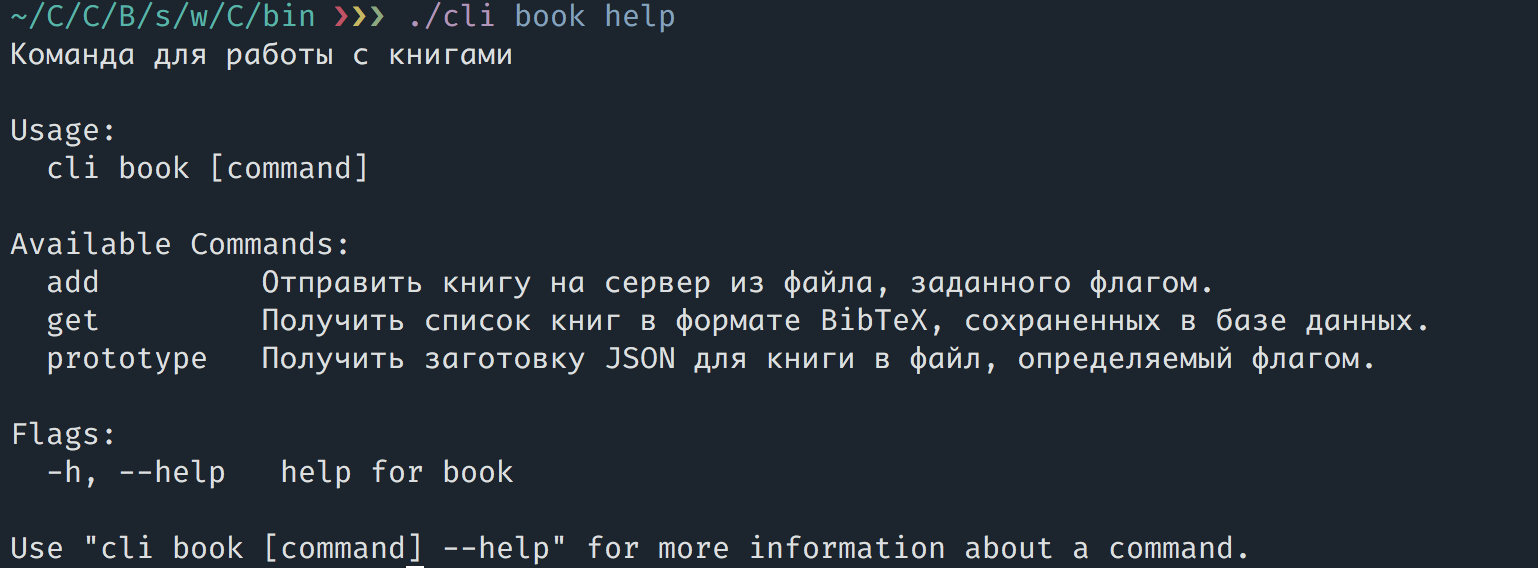
\includegraphics[width=1\linewidth]{help_book}}
\caption{Пример работы флага help для команды book}
\label{ris:help_book_example}
\end{figure}

\subsection*{Графический интерфейс}
\addcontentsline{toc}{subsection}{Графический интерфейс}

Как уже было сказано выше, графический интерфейс реализован в виде веб-сайта. Приложение было написано на языке TypeScript с 
использованием фреймворка Bootstrap.
Выбор фреймворка обусловлен тем, что он предоставляет продвинутый набор стилей и HTML-элементов, что позволяет 
легко и быстро настроить внешний вид веб-приложения.
В связи с тем, что единственный современный и поддерживаемый язык для написания веб-сайтов - это JavaScript, то 
из альтернатив ему можно использовать только языки, компилируемые в JavaScript. В частности, к таким языкам можно 
отнести язык TypeScript компании Microsoft и язык Kotlin, разрабатываемый компанией JetBrains, который имеет 
отдельный плагин для компиляции в JS-код. К сожалению, Kotlin является очень молодым языком, который находится в 
активной разработке, так что было решено использовать TypeScript\cite{TypeScript}. Преимуществом данного языка является то, что 
он является надмножеством JavaScript. Это означает, что любой код JavaScript является абсолютно корректным. Также 
важно отметить, что TypeScript поддерживает важные аспекты объектно-ориентированого программирования: по меньшей мере классы 
и инкапсуляцию. Но главным преимуществом этого языка является его строгая типизированность. 
Это облегчает разработку и позволяет писать более читаемый код по сравнению с JavaScript.

На рисунках ~\ref{ris:web_example_1} и ~\ref{ris:web_example_2} видно, приложение состоит из четырех логический частей. 

\begin{figure}[h!]
    \center{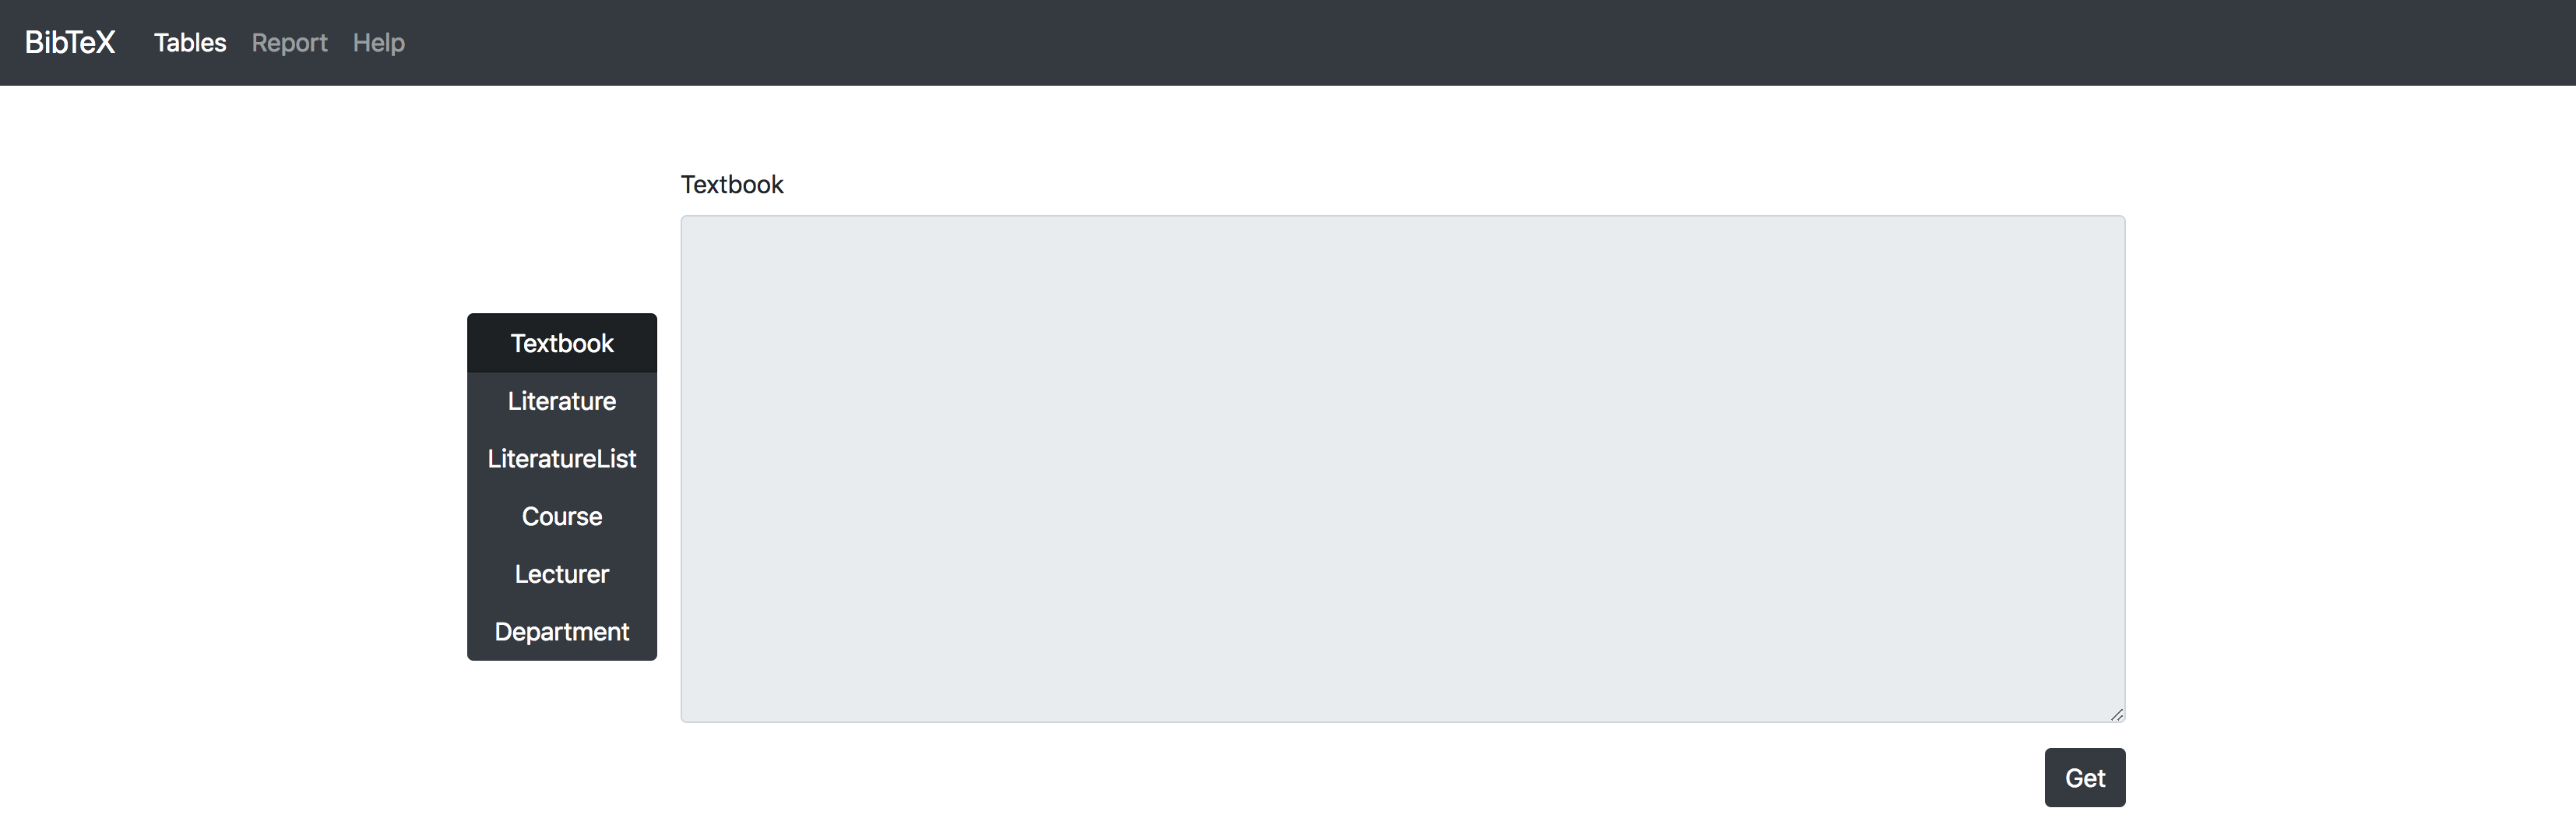
\includegraphics[width=0.8\linewidth]{web_example_1}}
    \caption{Верхняя часть веб-сайта}
    \label{ris:web_example_1}
\end{figure}

\begin{figure}[h!]
    \center{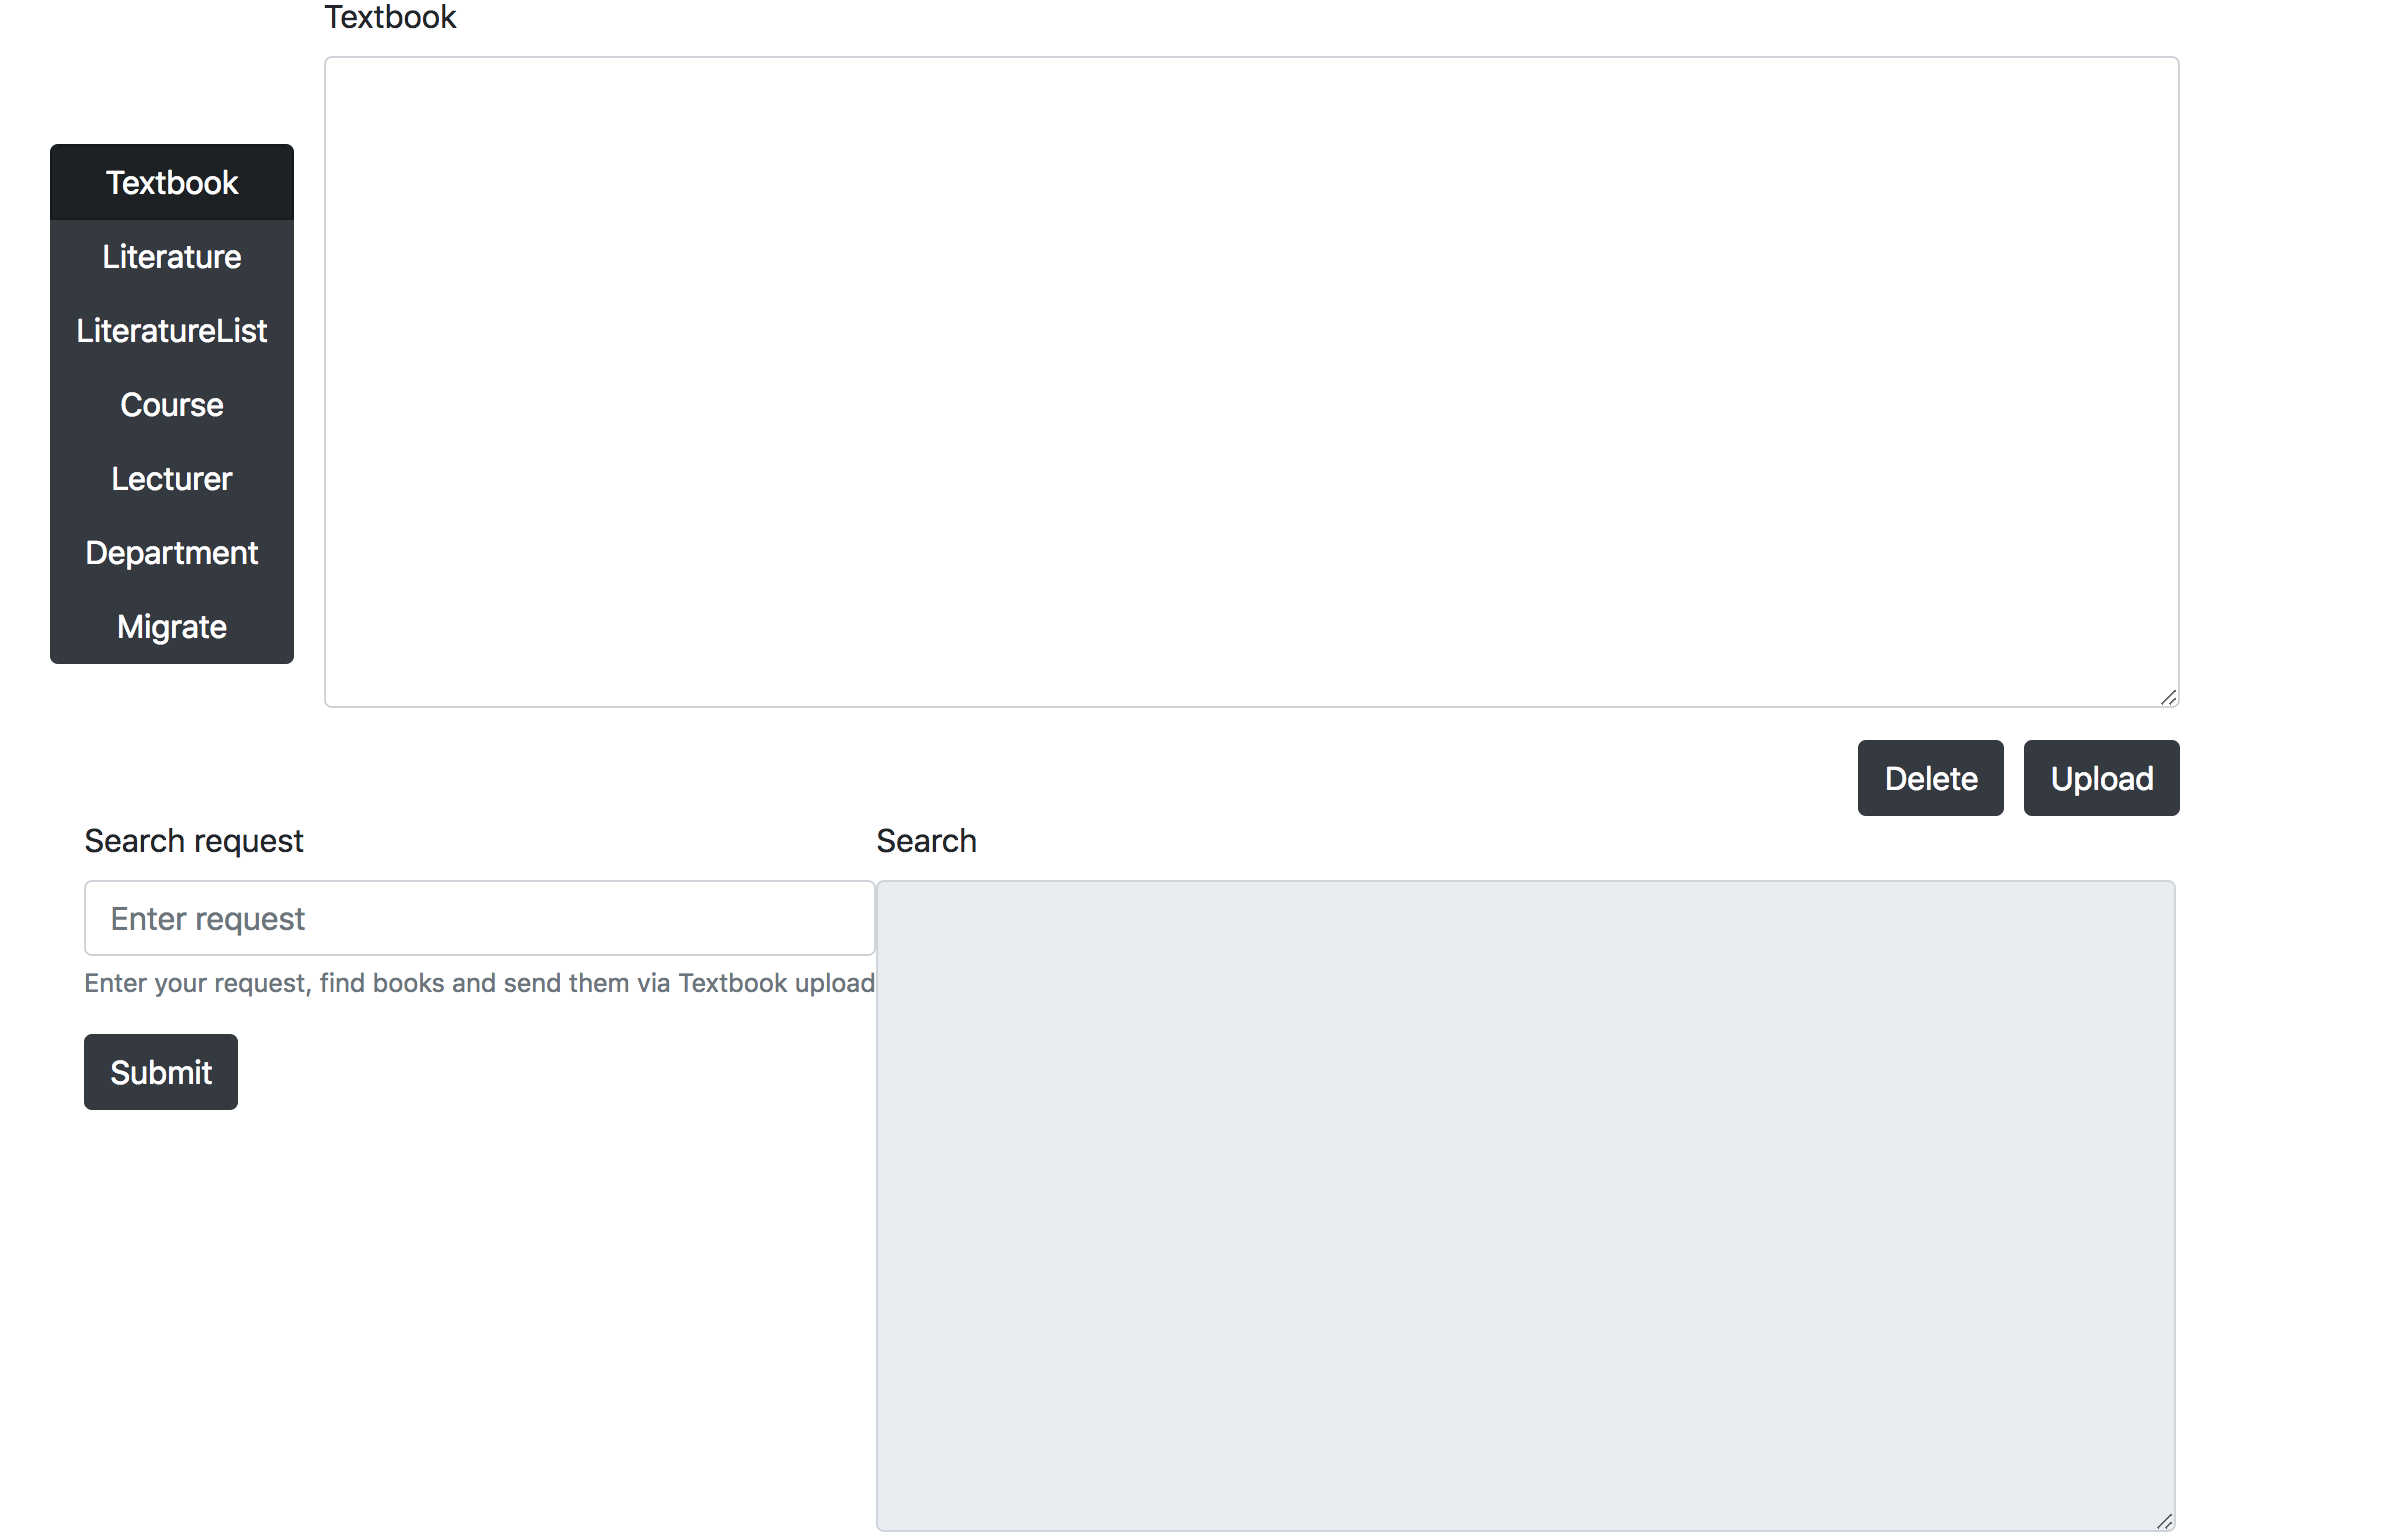
\includegraphics[width=0.8\linewidth]{web_example_2}}
    \caption{Нижняя часть веб-сайта}
    \label{ris:web_example_2}
\end{figure}

Первая - шапка сайта. Она содержит название 
приложения и ссылки на три страницы приложения: основную рабочую область, страницу генерации отчетов и страницу со 
справкой.

Вторая логическая часть - это большая недоступная для ввода область TextArea вместе с набором кнопок, 
отвечающих за переключение используемой таблицы. Эта часть нужна для получения данных, которые 
уже содержатся в базе данных для более удобного добавления новых записей в приложение.

Третья часть -- доступная для ввода область TextArea, в которую автоматически загружаются
JSON прототипы для текущего вида входных данных.

Заключительная область необходима для поиска необходимых книг в сервисе Google Books.

\subsection*{Серверная часть}
\addcontentsline{toc}{subsection}{Серверная часть}

Приложение написано на языке Go, его можно разделить на несколько модулей или пакетов, что и было сделано
в исходном коде программы. 

В первую очередь стоит отметить пакет \texttt{fetcher}, который отвечает за
поиск книг в сервисе Google Books. Он формирует запрос с помощью API-ключа и данных,
введенных пользователем, после чего отправляет его и получает ответ, а дальше возвращает его в необходимом
формате. Именно по этой причине для старта приложения необходимо вводить API-ключ.

Далее следует, пожалуй, самая крупная часть данного приложения: работа с базой данных. Как уже было упомянуто
выше, работа с ней ведется с использованием связки из модуля стандартной библиотеки \texttt{database/sql} и
драйвера \texttt{pq}. Пакет \texttt{database/sql} является исключительно интерфейсом, в то время как именно
драйвер реализует всю необходимую логику. Для их взаимодействия нужно добавить в файл оба этих пакета, используя команду
\texttt{import}.

Для начала будет правильным рассмотреть принципы работы с \texttt{database/sql}.
Подключение к СУБД происходит с помощью метода \texttt{sql.Open}.
Данный метод имеет два параметра:

\begin{itemize}
	\item Имя драйвера -- в данном случае это будет postgres.
	\item Конфигурационная строка -- набор пар ключ-значение, определяющее все параметры подключения. Например,
	      подключение к базе данных <<bibtex>> пользователя <<username>> к СУБД, находящейся на порту 8888, будет выглядеть
	      следующим образом: \texttt{"user=username port=8888 dbname=bibtex"}.
\end{itemize}

Метод \texttt{sql.Open} вернет структуру \texttt{sql.DB}, через которую будут происходить
все дальнейшие взаимодействия с СУБД, в частности, внесение и получение данных.

Следующим шагом стоит выполнить метод \texttt{DB.Ping}, который создает или восстанавливает подключение.
Это позволяет удостовериться, что все работает корректно. После этого СУБД готова к использованию в приложении.

В первую очередь при разработке были реализованы методы \texttt{insert} и \texttt{select} для всех таблиц.
Стоит отметить, что приложение рассчитано исключительно на использование из CLI и веб-приложения и не
предусматривает вставки нескольких записей за раз. \texttt{Select} внутри запроса сразу выполняет
необходимые объединения \texttt{join} для того, чтобы результат был максимально удобен для
использования пользователем.

Следующим шагом были разработаны методы для удаления из таблиц. Как уже было сказано выше,
было решено использовать каскадное удаление на стороне сервера. Для этого были использованы
транзакции. В пакете \texttt{database/sql} они представляются структурой \texttt{Tx}.
Если начинать использовать транзакции в удалении, то было бы логично начать использовать их везде, в том числе
и уже реализованных \texttt{insert} и \texttt{select}. Для этого был создан интерфейс языка Go, который можно увидеть в листинге ~\ref{sqlexecutable}.

\begin{lstlisting}[language=bash, caption = {Интерфейс унификации транзакций.}, captionpos=b, label={sqlexecutable}]
type SQLExecutable interface {
	Exec(string, ...interface{}) (sql.Result, error)
	Query(string, ...interface{}) (*sql.Rows, error)
	QueryRow(string, ...interface{}) *sql.Row
}
\end{lstlisting}

Этот интерфейс необходим для унификации используемых методов структур \texttt{sql.DB} и \texttt{sql.Tx}.
С использованием этого интерфейса стало возможно написание метода \texttt{getSQLExecutable}, который
возвращает структуру транзакции, если она была иницилизирована и обычную \texttt{sql.DB} в ином случае.

После этого достаточно все использования \texttt{sql.DB} заменить на метод \texttt{getSQLExecutable}.
Важно отметить, что для использования такого приема не требуется никакого изменения этих структур.
Дело в том, что, в отличии от, например, языка Java, для имплементации интерфейса структуре не
обязательно явно указывать список реализуемых интерфейсов. Компилятор способен сам определять, подходит
ли структура под выбранный интерфейс. В случае неудачи при компиляции будет выведена ошибка.

Теперь можно перейти непосредственно к методам удаления. Принцип их работы прост: в рамках одной
транзакции последовательно удалять все необходимые таблицы. Рассмотрим, например, последовательность действий
при удалении таблицы \texttt{Course}:

\begin{enumerate}
	\item удалить курс и получить список суррогатных ключей затронутых списков литературы,
	\item по суррогатным ключам удалить списки литературы, получить список суррогатных ключей
	      для связи многие-ко-многим с учебниками,
	\item по суррогатным ключам удалить все связи многие-ко-многим.
\end{enumerate}

Аналогично будет происходить со всеми остальными удалениями.

Последней проблемой в этой части приложения стала реализация обновления. Самым логичным поведением тут
является реализация политики <<при \texttt{insert} добавить новую запись, если записи с таким первичным ключом нет, 
обновить в ином случае>>. Это позволяет свести любые обновления к добавлениям, что уменьшает количество
кода и на сервере, и на клиентах. Но возникает проблема с тем, что такая возможность реализована во всех
СУБД немного по разному. Например, в SQLite для таких целей есть отдельная команда \texttt{replace}.
В PostgreSQL есть конструкция <<ON CONFLICT>>. Добавление в таблицу \texttt{Lecturer} с учетом этой конструкции можно
увидеть в листинге ~\ref{insert_lecturer}.

\begin{lstlisting}[language=bash, caption = {SQL запрос добавления записи в таблицу Lecturer}, captionpos=b, label={insert_lecturer}]
INSERT INTO schema.lecturer(
    lecturer_name, 
    lecturer_date_of_birth,
    lecturer_department_id, 
    lecturer_timestamp
    ) 
    VALUES ($1, $2, $3, $4)
        ON CONFLICT(lecturer_name, lecturer_date_of_birth) 
        DO UPDATE SET
            lecturer_department_id=
                EXCLUDED.lecturer_department_id,
            lecturer_timestamp=
                EXCLUDED.lecturer_timestamp,
            lecturer_is_deleted=
                FALSE;
\end{lstlisting}

При отладке этой части программы была обнаружена одна особенность языка Go, которая
сильно усложняет тестирование работоспособности приложения. Дело в том, что тип 
error, являющийся стандартным типом для ошибок, не предоставляет трассировку стека. Другими словами, по ошибке невозможно понять,
в каком месте программы она была вызвана в случае, если обработка этой ошибки делегируется
вызывающему методу. Дело в том, что тип error, которым представляются все ошибки в языке
Go, является всего лишь интерфейсом с одним методом \texttt{Error() string}, возвращающим текст ошибки.
Но, с другой стороны, такой подход позволяет реализовывать собственные типы ошибок,
что и было сделано данном приложении. Ошибка представляется типом \texttt{Error}, который можно увидеть в листинге ~\ref{error}:

\begin{lstlisting}[language=bash, caption = {Стурктура Error.}, captionpos=b, label={error}]
type Error struct {
	Message       string
	StackTrace    string
	DatabaseError *pq.Error
}
\end{lstlisting}

Перечислим назначение каждого поля.

\begin{enumerate}
	\item \texttt{Message} -- текстовое сообщение об ошибке,
	\item \texttt{StackTrace} -- трассировка ошибки, созданная на основе метода \texttt{runtime.Stack} пакета \texttt{runtime},
	\item \texttt{DatabaseError} -- указатель на ошибку драйвера \texttt{pq}, работающего с PostgreSQL. Указатель равен \texttt{nil}
	      в случае, если ошибка произошла не в драйвере.
\end{enumerate}

Теперь следует описать принципы работы программного интерфейса. В разработанном приложении используется HTTP-сервер из стандартной
библиотеки языка Go. Использовать этот пакет очень просто: необходимо добавить необходимый метод с нужной сигнатурой и
URL-строку в сервер с помощью метода \texttt{http.HandleFunc}. В этой сигнатуре функция должна принимать два аргумента:
\texttt{http.ResponseWriter}, который предназначен для отправки ответа клиенту и \texttt{http.Request}, содержащий информацию
о поступившем запросе. В приложении на каждый запрос первым делом выполняется проверка входных данных, если таковые имеются.
По большей части это проверка на наличие тела запроса, если оно должно присутствовать.

Также при обработке каждого запроса в ответ добавляется заголовок \texttt{Access-Control-Allow-Origin}, который необходим
для того, чтобы при использовании этого API браузером все работало корректно. Без этого хэдера браузеры просто блокируют запросы
к серверу. Согласно документации компании <<Mozilla>>\cite{Access-Control-Allow-Origin}, этот заголовок позволяет
установить, с какими сайтами сервер умеет работать, а с какими не умеет. Например, в него можно записать \texttt{https://developer.mozilla.org},
что означает, что сервер умеет работать только с одним этим сайтом. Если значение будет \texttt{*}, тогда сервер будет работать с абсолютно
любым клиентом.

Для каждой таблицы имеется следующий набор методов:

\begin{enumerate}
	\item получение содержимого таблицы,
	\item добавление записи в таблицу,
	\item удаление из таблицы,
	\item получение прототипа JSON-файла для записи таблицы.
\end{enumerate}

Также сервер имеет три дополнительных метода помимо описанной структуры. 
Первый метод выполняет миграцию списка литературы с одного года на другой.
Второй нужен для получения прототипа JSON-файла миграции, а третий выполняет генерацию отчета
и записывает его на клиент в виде текстового файла. В случае веб-версии происходит создание текстового файла в формате \texttt{.bib}, который
сохраняется в загрузки.